\chapter{Конструкторская часть}

В данном разделе будут представлены схемы последовательной и конвейерной обработки строк. Будут описаны типы и структуры данных, используемые для реализации, а также структура разрабатываемого программного обеспечения. Кроме того, будут выделены классы эквивалентности для тестирования.

\section{Разработка алгоритмов}

На рисунке \ref{img:linear} представлена схема последовательной обработки набора строк, на рисунке \ref{img:threads} - параллельного. Схемы алгоритмов работы лент конвейера показаны на рисунках \ref{img:first}-\ref{img:third}. Схема алгоритма удаления пробелов в строке представлена на рисунке \ref{img:spaces}, перевода регистра симовлов строки в другой - на рисунке \ref{img:register}, определение строки-палиндрома - \ref{img:palindrome}.

\begin{figure}[H]
	\begin{center}
		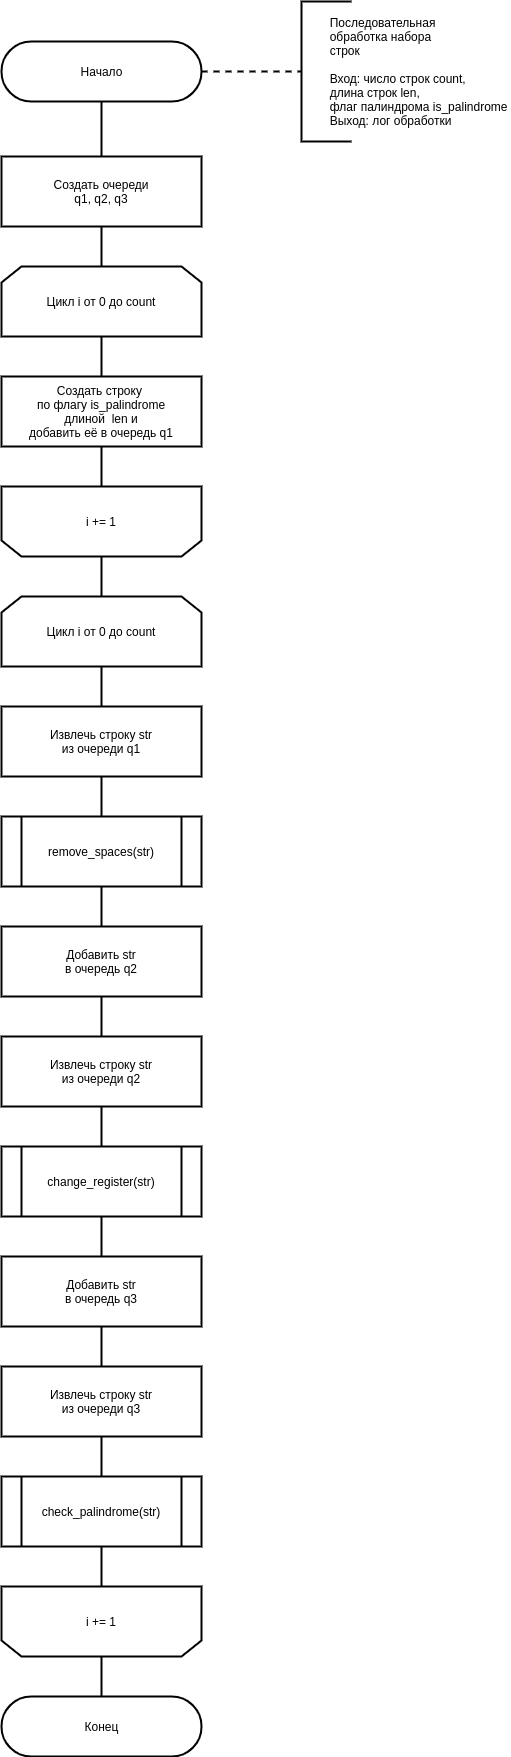
\includegraphics[scale=0.4]{img/linear.png}
	\end{center}
	\captionsetup{justification=centering}
	\caption{Последовательная обработка набора строк}
	\label{img:linear}
\end{figure}

\begin{figure}[H]
	\begin{center}
		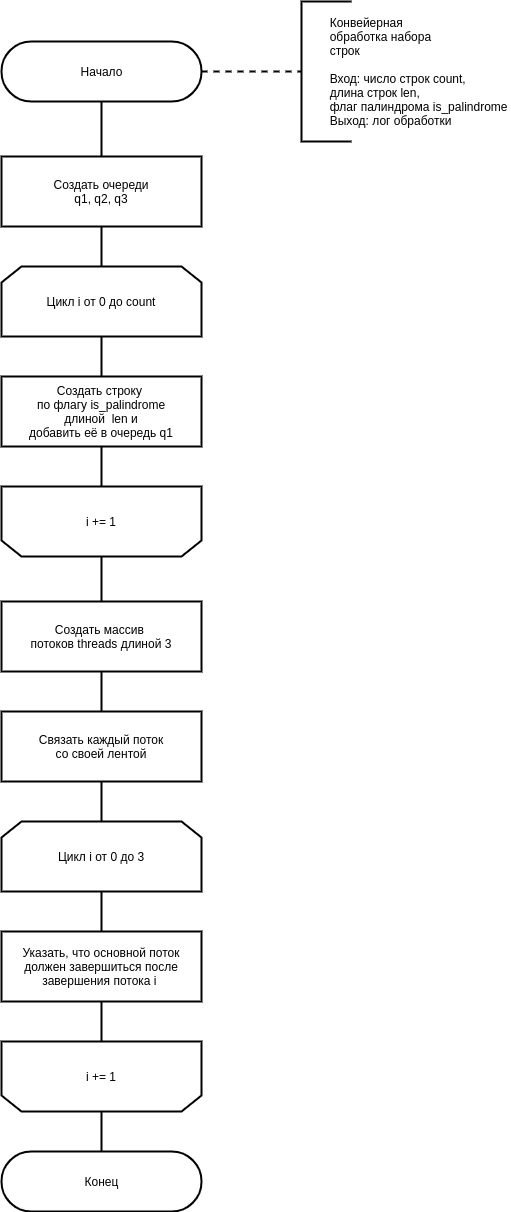
\includegraphics[scale=0.5]{img/threads.png}
	\end{center}
	\captionsetup{justification=centering}
	\caption{Конвейерная обработка набора строк}
	\label{img:threads}
\end{figure}

\begin{figure}[H]
	\begin{center}
		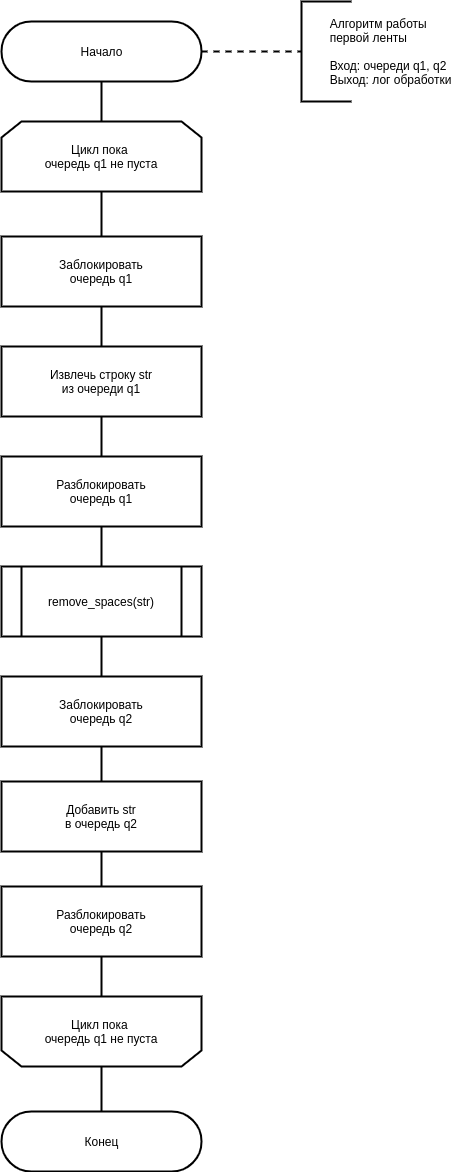
\includegraphics[scale=0.5]{img/first.png}
	\end{center}
	\captionsetup{justification=centering}
	\caption{Алгоритм работы первой ленты}
	\label{img:first}
\end{figure}

\begin{figure}[H]
	\begin{center}
		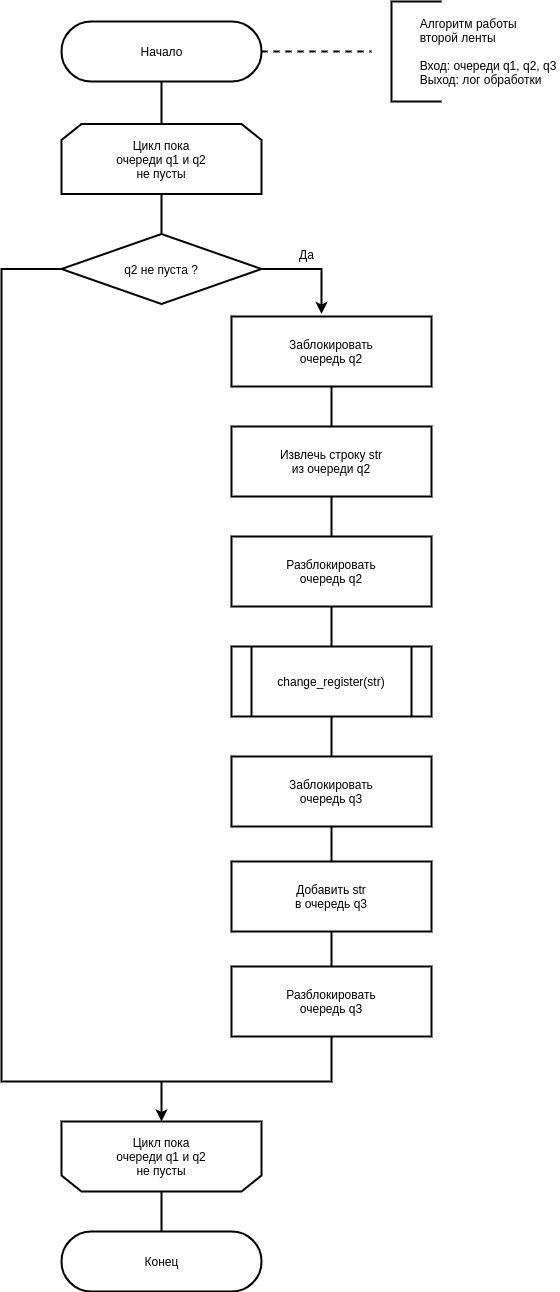
\includegraphics[scale=0.5]{img/second.png}
	\end{center}
	\captionsetup{justification=centering}
	\caption{Алгоритм работы второй ленты}
	\label{img:second}
\end{figure}

\begin{figure}[H]
	\begin{center}
		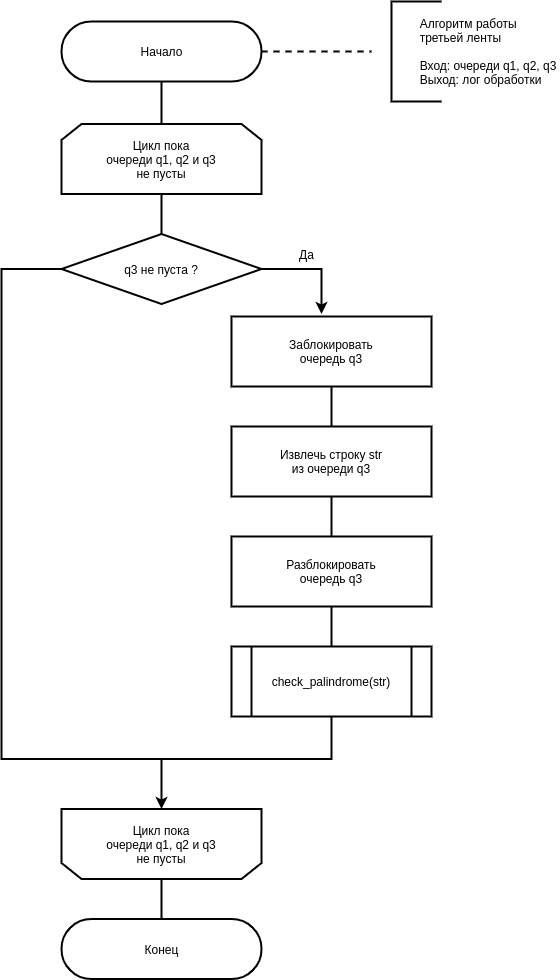
\includegraphics[scale=0.5]{img/third.png}
	\end{center}
	\captionsetup{justification=centering}
	\caption{Алгоритм работы третьей ленты}
	\label{img:third}
\end{figure}

\begin{figure}[H]
	\begin{center}
		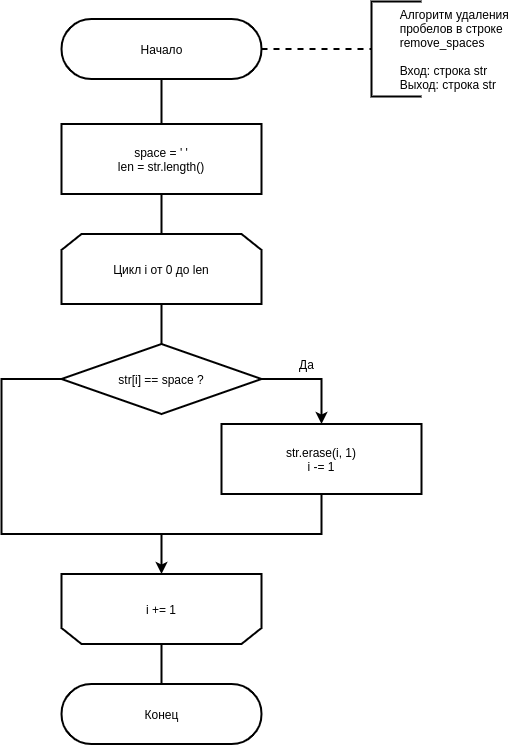
\includegraphics[scale=0.6]{img/spaces.png}
	\end{center}
	\captionsetup{justification=centering}
	\caption{Алгоритм удаления пробелов в строке}
	\label{img:spaces}
\end{figure}

\begin{figure}[H]
	\begin{center}
		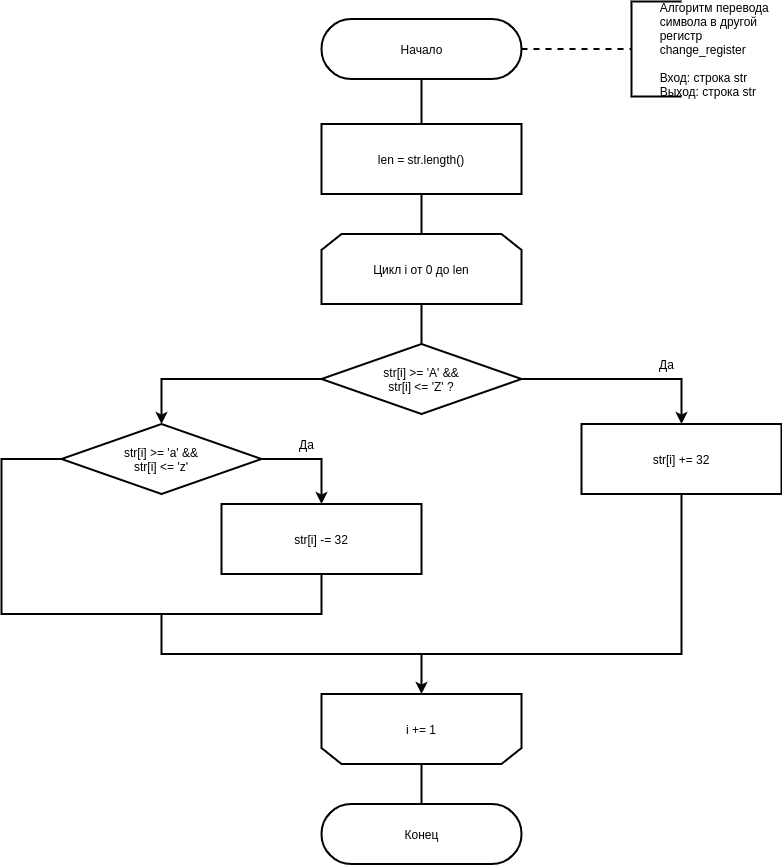
\includegraphics[scale=0.6]{img/register.png}
	\end{center}
	\captionsetup{justification=centering}
	\caption{Алгоритм перевода регистров символов строки}
	\label{img:register}
\end{figure}

\begin{figure}[H]
	\begin{center}
		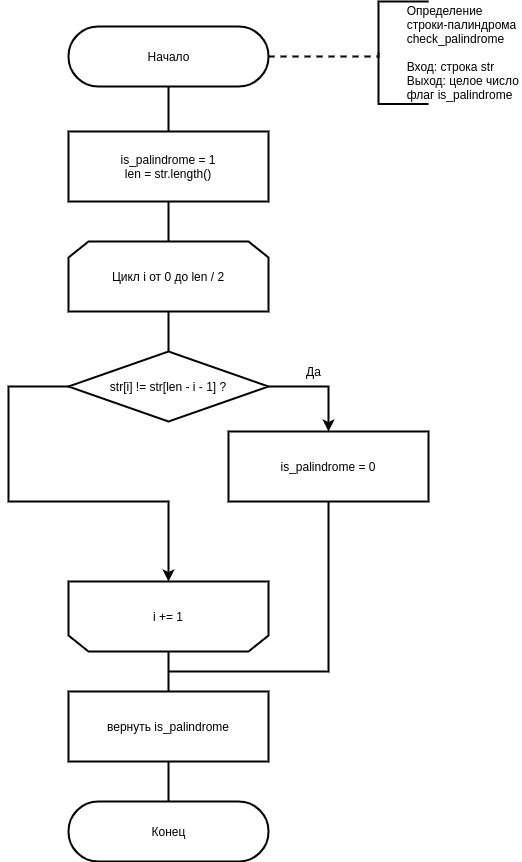
\includegraphics[scale=0.6]{img/palindrome.png}
	\end{center}
	\captionsetup{justification=centering}
	\caption{Алгоритм определения строки-палиндрома}
	\label{img:palindrome}
\end{figure}

\section{Описание используемых типов и структур данных}

Для реализации набора строк будут использованы следующие типы:
\begin{itemize}
	\item тип $int$ для числа строк в наборе и для длины строки;
	\item $std::string$ для строки.
\end{itemize}

Для представления очередей будет использован тип $std::queue$, для потоков - $std::thread$.

\section{Структура разрабатываемого ПО}

При реализации разрабатываемого программного обеспечения будет использоваться метод структурного программирования. Для взаимодействия с пользователем в функции $int  main(void)$ будет реализовано меню, при помощи которого будут вызываться последовательная и параллельная обработка строк и функции сравнительного анализа. 

Для работы со строками будут разработаны следующие функции, принимающие на вход ссылку на строку:

\begin{itemize}
	\item процедура создания строки, состоящей из случайных символов из допустимого набора, входными параметрами процедуры также являются длина строки и флаг для создания строки-палиндрома; 
	\item создание графа со случайными весами ребер, выходным параметром функции является сгенерированная матрица смежности;
	\item процедура удаления пробелов;
	\item процедура перевода в другой регистр;
	\item функция определения строки-палиндрома.
\end{itemize}

Для организации обработки набора строк будут реализованы:

\begin{itemize}
	\item процедуры последовательной и конвейерной обработки, у которых на входе - число строк, их длина и флаг для создания строки-палиндрома;
	\item процедуры работы с очередями, входными параметрами которых являются ссылки на очереди.
\end{itemize}

Для сравнительного анализа будут реализованы:

\begin{itemize}
	\item процедуры логирования, у которых на входе - ссылка на строку и номера ленты и задачи;
	\item процедуры замеров времени;
	\item функция графического представления замеров времени, у которой на входе - массив временных значений, на выходе - его графическое представление.
\end{itemize}

\section{Классы эквивалентности при тестировании}

Для тестирования разрабатываемой программы будут выделены следующие классы эквивалентности:

\begin{itemize}
	\item некорректная длина строки (не число или неположительное число);
	\item некорректный ввод числа строк (не число или неположительное число);
	\item корректный ввод всех параметров.
\end{itemize}

\section{Вывод}

Были представлены схемы обработки строк. Были указаны типы и структуры данных, используемые для реализации, и описана структура разрабатываемого программного обеспечения. Также были выделены классы эквивалентности для тестирования ПО.
